\documentclass[preview]{standalone}

\usepackage{amsmath}
\usepackage{amssymb}
\usepackage{parskip}
\usepackage{fullpage}
\usepackage{hyperref}
\usepackage{tikz}
\usepackage{pgfplots}
\usepackage{wrapfig}
\usepackage{stellar}
\usepackage{definitions}
\usepackage{bettelini}

\usetikzlibrary{positioning, arrows.meta} 

\begin{document}

\id{integration}
\genpage

\section{Indefinite Integrals}

\subsection{Definitions}

\begin{snippetdefinition}{primitive-function-definition}{Primitive function}
    Given a \function \(f(x)\colon I \to \mathbb{R}\)
    where \(I\) is an interval, an \textit{anti-derivative} or \textit{primitive}
    is any \function \(F(x)\) differentiable in \(I\) such that
    \[
        \frac{dF}{dx} = f(x)
    \]
\end{snippetdefinition}

\begin{snippetdefinition}{indefinite-integral-definition}{Indefinite integral}
    The operator to find a primitive function is called the \textit{indefinite integral}
    \[
        \integral[f(x)][x]=F(x)+C,
        \quad C\in\realnumbers
    \]
    The function to integrate (integrand) is delimited by the integral symbol \(\int\)
    and a differential of the variable of integration \(dx\).
\end{snippetdefinition}

\begin{snippet}{indefinite-inegral-expl}
    A \function has infinitely many primitives, hence the \(+ C\) term. This essentially
    means that the derivative of a \function is the same when the function is shifted
    up or down, the rate of change is the same. By reversing the process we don't know
    the up or down shift of the original function.
    \[
        f(x)=\integral[\frac{df}{dx}][x] + C
    \]
    for some specific \(C\).
\end{snippet}

\subsection{Properties}

\begin{snippet}{indefinite-integral-properties}
If \(k\) is a constant
\[
    \integral[kf(x)][x] = k \integral[f(x)][x]
\]

\[
    \integral[f(x) \pm g(x)][x] = \integral[f(x)][x] \pm \integral[g(x)][x]
\]
\end{snippet}

\subsection{Substitution Rule}

\begin{snippettheorem}{substitution-rule}{Substitution Rule}
    Given an integral in the form
    \[
        \integral[f(g(x))g'(x)][x]
    \]
    Let
    \[
        u = g(x)
    \]
    The differential of u is then
    \[
        du=g'(x)dx
    \]
    meaning that we can rewrite the integral as
    \[
        \integral[f(u)][u] = F(u) + C = F(g(x)) + C
    \]
\end{snippettheorem}

\subsection{Integration By Parts}

\begin{snippettheorem}{integration-by-parts}{Integration by parts}
    Let \(f(x)\) and \(g(x)\) be \function[functions]
    \[
        \int f(x)g'(x)\,dx = f(x)g(x) - \int f'(x)g(x)\,dx
    \]
\end{snippettheorem}

\begin{snippetproof}{integration-by-parts-proof}{integration-by-parts}{Integration by parts}
    Starting from the product rule
    \[
        \frac{d}{dx}\big(f(x)g(x)\big)=f'(x)g(x)+f(x)g'(x)
    \]
    if we integrate both parts we get
    \begin{align*}
        f(x)g(x)+C&=\int f'(x)g(x)\,dx+\int f(x)g'(x)\,dx \\
        \int f(x)g'(x)\,dx &= f(x)g(x)+C - \int f'(x)g(x)\,dx 
    \end{align*}
    Since the indefinite integral of \(f'(x)g(x)\) is equal to some function plus an arbitrary constant, we can ignore the \(+C\) term.
    \[
        \int f(x)g'(x)\,dx = f(x)g(x) - \int f'(x)g(x)\,dx
    \]
\end{snippetproof}

\section{Definite Integrals}

\subsection{Area Problem}

\begin{snippet}{area-problem-illustration}
    \begin{wrapfigure}{l}{10cm}
        \begin{center}
            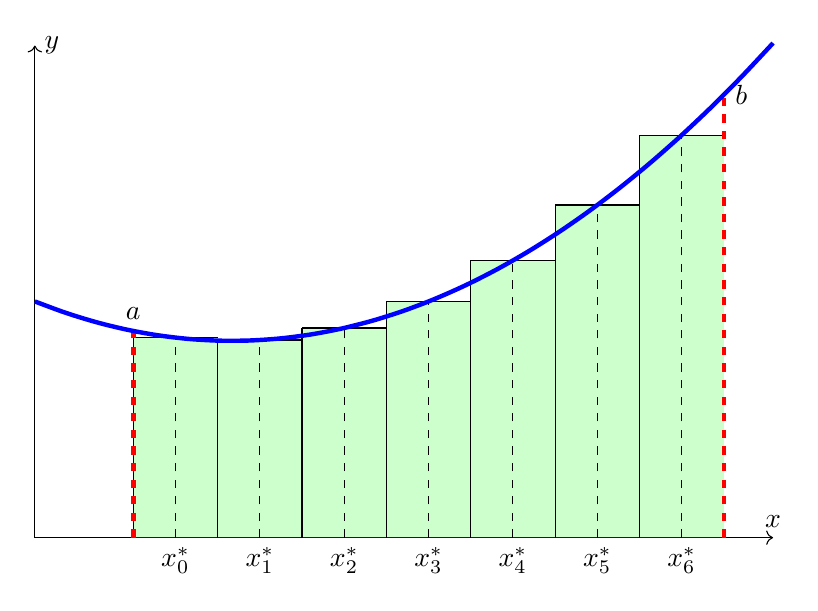
\begin{tikzpicture}[
                scale=1.25,
                declare function={
                    func(\x) = 0.1 * (\x - 2) * (\x - 2) + 2;
                    Width=7.5;
                    Height=5;
                    A = 1;
                    B = 7;
                    N = 7;
                    Delta = {(B-A) / N};
                }
            ]
                \draw[->] (0, 0) -- (0, Height) node[right] {\(y\)};
                \draw[->] (0, 0) -- (Width, 0) node[above] {\(x\)};
        
                \pgfmathtruncatemacro\END{N-1}
                \foreach \x in {0,1,...,\END} {
                    % rectangle
                    \fill [green, opacity=0.2]
                        ({A + Delta * \x}, 0) rectangle ({A + Delta * (\x+1)}, {func(A + Delta * (\x + 0.5))});
                    
                    \draw[-] ({A + Delta * \x}, 0)
                        -- ({A + Delta * \x}, {func(A + Delta * (\x + 0.5))});

                    \draw[-, dashed] ({A + Delta * (\x + 0.5)}, 0)
                        node[below] {\(x_{\x}^*\)}
                        -- ({A + Delta * (\x + 0.5)}, {func(A + Delta * (\x + 0.5))});

                    % line over rectangle
                    \draw[-] ({A + Delta * \x}, {func(A + Delta * (\x + 0.5))})
                        -- ({A + Delta * (\x+1)}, {func(A + Delta * (\x + 0.5))});
                }
        
                \draw[-, dashed, red, ultra thick] (A, 0) -- (A, {func(A)}) node[above, black] {\(a\)};
                \draw[-, dashed, red, ultra thick] (B, 0) -- (B, {func(B)}) node[right, black] {\(b\)};
        
                \draw[domain=0:Width, smooth, variable=\x, blue, ultra thick] plot ({\x}, {func(\x)});
            \end{tikzpicture}
        \end{center}
    \end{wrapfigure}

    We want to find the signed area between \(f(x)\) and the \(x\)-axis between
    the interval \([a;b]\).\\
    One way to do it would be by dividing the area into \(n\) rectangles, each of width
    \[
        \Delta x = \frac{b-a}{n}
    \]
    The height of each triangle is given by \(f(x_k^*)\).
    The area under the curve is approximately
    \[
        A \approx \sum_{k=0}^{n-1}f(x_k^*)\Delta x
    \]
    Notice that the position of \(x_k^*\) within the base of each rectangle controls the type of
    the approximation of the area under the curve.
    By moving \(x_k^*\) within the base we may achieve an approximation by abundance
    or defect.
    The type of approximation does not matter when we let \(n\to \infty\).
    As the amount of rectangles approaches infinity, the approximation approaches
    the exact value of the area.
    \[
        A = \lim_{n\to\infty} \sum_{k=0}^{n}f(x_k^*)\Delta x
    \]
    \wrapfill
\end{snippet}

\subsection{Definition}

\begin{snippet}{definite-integral-definition}
Given a \function \(f(x)\) continuous on the interval \([a;b]\), we divide the interval
into \(n\) rectangles of width \(\Delta x = \frac{b-a}{n}\) and height \(f(x_k^*)\).
The definitive interval of \(f(x)\) from \(a\) to \(b\) is
\[
    \integral[a][b][f(x)][x] = \lim_{n\to \infty} \sum_{k=0}^{n} f(x_k^*)\Delta x
\]
\end{snippet}

\subsection{Properties}

\begin{snippet}{definite-integral-properties}
    \[
        \integral[a][b][f(x)][x] = -\integral[b][a][f(x)][x]
    \]
    If \(k\) is constant
    \[
        \integral[a][b][cf(x)][x] = c\integral[a][b][f(x)][x]
    \]
    \[
        \integral[a][b][f(x)\pm g(x)][x] = \integral[a][b][f(x)][x] \pm \integral[a][b][g(x)][x]
    \]
    \[
        \integral[a][a][f(x)][x] = 0
    \]
\end{snippet}

\subsection{Fundamental Theorem of Calculus}

\begin{snippettheorem}{fundamental-theorem-of-calculus}{Fundamental Theorem of Calculus}
    A primitive function \(F(x)\) (with \(C=0\), thus passing through the origin) represents the area
    from \(0\) to \(x\) of \(f(x)\).

    Let \(f(x)\) be continuous on the interval \(I=[a;b]\) and \(F(x)\) any primitive of \(f(x)\),
    then \(F(x)\) is also continuous on \(I\) and
    \[
        \integral[0][x][f(t)][t] = F(x)
    \]
    and
    \[
        \integral[a][b][f(x)][x] = F(b) - F(a)
    \]
    This also means that
    \[
        f(x)=\integral[0][x][f'(t)][t]
    \]
    or
    \[
        \frac{d}{dx}\integral[a][x][f(t)][t]=f(x)
    \]
\end{snippettheorem}

\begin{snippetcorollary}{fundamental-calculus-theorem-corollary-1}{Non-constant integral limits derivative}
    When the upper or lower limit is not constant,
    \begin{align*}
        \frac{d}{dx} \integral[v(x)][u(x)][f(t)][t]
        &= \frac{d}{dx} \left[ F(u(x)) - F(v(x)) \right] \\
        &= u'(x)f(u(x)) - v'(x)f(v(x))
    \end{align*}
\end{snippetcorollary}

\section{Average Function Value}

\begin{snippettheorem}{average-function-value}{Average Function Value}
    The average value of a continuous function \(f(x)\) over the interval \([a;b]\) is given by
    \[
        f_\text{avg} = \frac{1}{b-a} \integral[a][b][f(x)][x]
    \]
\end{snippettheorem}

\section{Mean Value Theorem}

\begin{snippettheorem}{mean-value-theorem}{Mean Value Theorem}
    If \(f(x)\) is a continuous function on \(I=[a;b]\), \(f(x)\) will at some point in \(I\)
    reach its average value, meaning
    \[
        \exists c \suchthat f(c) = \frac{1}{b-a} \integral[a][b][f(x)][x]
    \]
\end{snippettheorem}

\section{Area Between Functions}

\begin{snippet}{area-between-functions-illustration}
    \begin{wrapfigure}{l}{7.5cm}
        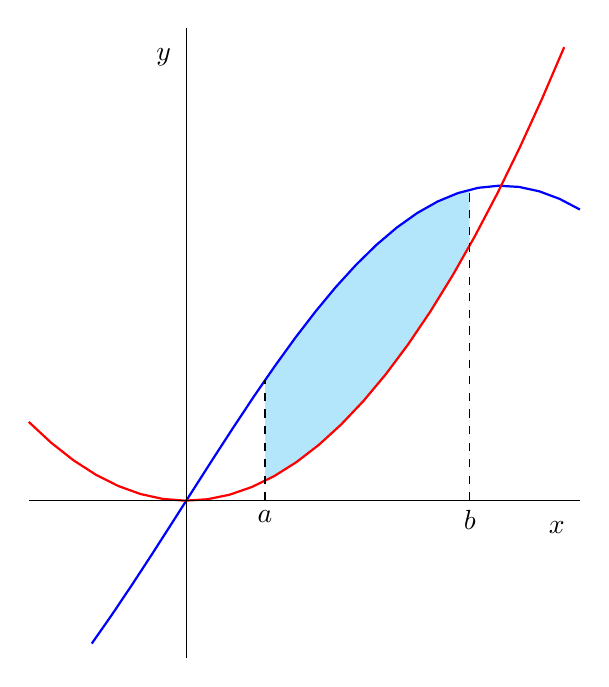
\begin{tikzpicture}[x=4cm, y=4cm, >=Stealth, declare function={
            func1(\x) = sin(3.14*\x/2 r);
            func2(\x) = \x*\x;
            a=0.25;
            b=0.9;
        }]
            % area under func1 
            \fill[cyan!30!white] plot[domain=a:b] (\x,{func1(\x)}) -- plot[domain=b:a] (\x,{0}) -- cycle;
            

            % area under func2
            \fill[white] plot[domain=a:b] (\x,{func2(\x)}) -- plot[domain=b:a] (\x,{0}) -- cycle;
            
            % func1
            \draw[blue, -, thick] plot[domain=-0.3:1.25] (\x,{func1(\x)});
            
            % func2
            \draw[red, -, thick]  plot[domain=-0.5:1.2] (\x,{func2(\x)});

            \draw[-, dashed] (a, 0) node[below] {\(a\)} -- (a, {func1(a)});
            \draw[-, dashed] (b, 0) node[below] {\(b\)} -- (b, {func1(b)});

            \draw[-] (-.5,0) -- (1.25, 0)
                node[below left=4pt and 2pt] {\(x\)};
            \draw[-] (0,-.5) -- (0,1.5)
                node[below left=4pt and 2pt] {\(y\)};
        \end{tikzpicture} 
    \end{wrapfigure}

    Given a \function \(y=f(x)\) and \(y=g(x)\), the area enclosed by the two functions
    in the interval \(I=[a;b]\) is given by
    \[
        A=\integral[a][b][f(x)-g(x)][x]
    \]
    assuming that \(f(x)\geq g(x)\) when \(x\in I\). \\
    Note that \(A\geq 0\). \\
    If \(f(x)<g(x)\) for some \(x\in I\) this formula won't work. However, it is still
    possible to split the integral into multiple integrals at every point where \(f(x) - g(x)\) changes sign.
    To remove the sign contraint we could say
    \[
        A = \integral[a][b][|f(x)-g(x)|][x]
    \]
    \wrapfill

    \begin{wrapfigure}{l}{7.5cm}
        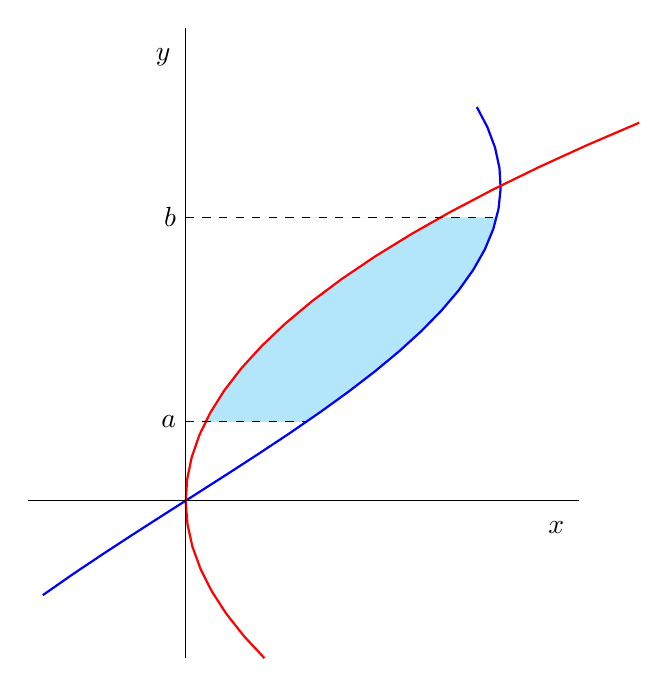
\begin{tikzpicture}[x=4cm, y=4cm, >=Stealth, declare function={
            func1(\x) = sin(3.14*\x/2 r);
            func2(\x) = \x*\x;
            a=0.25;
            b=0.9;
        }]
            % area under func1 
            \fill[cyan!30!white] plot[domain=a:b] ({func1(\x)},\x) -- plot[domain=b:a] ({0}, \x) -- cycle;
            

            % area under func2
            \fill[white] plot[domain=a:b] ({func2(\x)}, \x) -- plot[domain=b:a] ({0}, \x) -- cycle;
            
            % func1
            \draw[blue, -, thick] plot[domain=-0.3:1.25] ({func1(\x)}, \x);
            
            % func2
            \draw[red, -, thick]  plot[domain=-0.5:1.2] ({func2(\x)}, \x);

            \draw[-, dashed] (0, a) node[left] {\(a\)} -- ({func1(a)}, a);
            \draw[-, dashed] (0, b) node[left] {\(b\)} -- ({func1(b)}, b);

            \draw[-] (-.5,0) -- (1.25, 0)
                node[below left=4pt and 2pt] {\(x\)};
            \draw[-] (0,-.5) -- (0,1.5)
                node[below left=4pt and 2pt] {\(y\)};
        \end{tikzpicture} 
    \end{wrapfigure}

    The same thing applies when we have functions in the form \(x=f(y)\) and \(x=g(y)\)
    and we want to find the areas enclosed by the functions when \(y\in [d;c]\)
    \[
        A=\integral[d][c][|f(y)-g(y)|][y]
    \]

    \wrapfill
\end{snippet}

\section{Volume of solid revolutions}

\begin{snippet}{volume-of-solid-revolutions-illustration}
    A solid of revolution is a solid made by rotating about an axis a \function
    on an interval \([a;b]\).

    \begin{minipage}{0.5\textwidth}
        \begin{tikzpicture}[
            scale=0.75,
            declare function={
                func(\x) = 0.1 * (\x - 2) * (\x - 2) * sin(\x r) + 2;
            }
        ]

            \draw[-] (0,0) -- (9,0) node [above] {\(x\)};
            \draw[-] (0,-2) -- (0,6) node [above] {\(y\)};
            \draw[domain=0:9, smooth, variable=\x, blue, thick] plot ({\x}, {func(\x)});
        \end{tikzpicture}
    \end{minipage}
    \begin{minipage}{0.5\textwidth}
        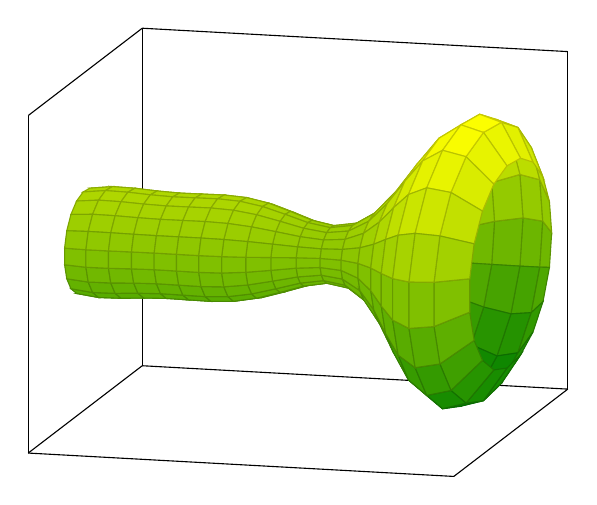
\begin{tikzpicture}[
            declare function={
                func(\x) = 0.1 * (\x - 2) * (\x - 2) * sin(\x r) + 2;
            }
        ]
            \begin{axis}[
                ticks=none,
                colormap/greenyellow,
                view={15}{15}
                ]    
        
                \addplot3[
                    surf,
                    shader=faceted,
                    samples=20,
                    domain=0:9,y domain=0:2*pi,
                    z buffer=sort]
                (x,{func(x) * cos(deg(y))}, {func(x) * sin(deg(y))});
        
            \end{axis}
        \end{tikzpicture}
    \end{minipage}
\end{snippet}

\subsection{Simple revolutions}

\begin{snippet}{simple-revolutions}
Let's start by assuming a rotation aroud the \(x\)-axis of a \function \(y=f(x)\) on \([a;b]\).
we divide the interval into \(n\) subsections of width \(\Delta x = \frac{b-a}{n}\).
For each section we then choose a point \(x^*_k\).
Every subsection is the height of a disk.
The volume is therefore given by the sum of volumes of every disk.
\[
    V \approx \sum_{k=0}^n A(x_k^*) \Delta x
\]
where \(A(x_k^*)\) is the area of the base of the disk of the \(k\)-th subsection. \\
Since we are summing over disks the area of the base is given by
\[
    A=\picircle \cdot {[f(x)]}^2
\]

If we divide the interval into ever smaller sections, the volume becomes exact
\begin{align*}
    V &= \lim_{n\to\infty} \sum_{k=0}^n A(x_k^*) \Delta x
    \\
    &= \integral[a][b][A(x)][x]
\end{align*}

The same approach works for a rotation around the \(y\)-axis.
\[
    V = \integral[a][b][A(y)][y]
\]
where \(A=\picircle \cdot {[f(y)]}^2\)
\end{snippet}

\subsection{Hollow volumes}

\begin{snippet}{hollow-volumes}
When the volume is obtained by rotating an area bounded by two functions, the volume
is partially hollow. This can also happen with a single function.
In this case we can obtain the volume as \(\textbf{outer volume} - \textbf{inner volume}\)
or by summing a set of annuluses rather than disks.
Using annuluses,
\[
    A = \picircle \left[
        {(\text{outer radius})}^2 - {(\text{inner radius})}^2    
    \right]
\]
When we have disks, \(\text{inner radius}=0\). More complex shapes may
require other area functions.
\end{snippet}

\subsection{Other axis}

\begin{snippet}{revolution-integral-other-axis}
When we are rotating a \function about \(x=a\) or \(y=a\)
we need to change the area function accordingly, therefore
usually adjusting the \textbf{outer radius} and \textbf{inner radius}
variables.
\end{snippet}

\subsection{Method of cylinders}

\begin{snippet}{method-of-cylinders}
Sometimes it is tricky or impossible to integrate the volume using disks or annuluses.
We can also cover the volume by using the area of an empty cylinder. In this case we would have
\[
    A = 2\picircle rh
\]
where \(r\) is the radius of the cylinder ad \(h\) is the height of the cylinder.
% https://tutorial.math.lamar.edu/Classes/CalcI/VolumeWithCylinder.aspx
\end{snippet}

\end{document}